\documentclass[11pt]{article}
\usepackage[T1]{fontenc}
\usepackage[utf8]{inputenc}
\usepackage[letterpaper]{geometry}

\usepackage{graphicx}
\usepackage{mathpazo}

\usepackage{amsmath}
\usepackage{amsfonts}
\usepackage{bm}
\usepackage{siunitx}
\usepackage{cancel}
\usepackage{float}
\usepackage{empheq}
\usepackage[most]{tcolorbox}

% Sexy yellow highlighted boxed equations!
\newtcbox{\mymath}[1][]{%
	nobeforeafter, math upper, tcbox raise base,
	enhanced, colframe=black!30!black,
	colback=yellow!30, boxrule=1pt,
	#1}

% Hyperlinks with decent looking default colors.
\usepackage{hyperref}
\usepackage{xcolor}
\hypersetup{
	colorlinks,
	linkcolor={red!50!black},
	citecolor={blue!50!black},
	urlcolor={blue!80!black}
}

% For those sexy spaced low small caps from classic-thesis!
\usepackage{microtype}
\usepackage{textcase}
\DeclareRobustCommand{\spacedlowsmallcaps}[1]{%
	\textls[80]{\scshape\MakeTextLowercase{#1}}%
}

% Replaced mathpazo \sum symbol with computer modern's.
\DeclareSymbolFont{cmlargesymbols}{OMX}{cmex}{m}{n}
\let\sumop\relax
\DeclareMathSymbol{\sumop}{\mathop}{cmlargesymbols}{"50}

% Force indent command.
\newcommand{\forceindent}{\leavevmode{\parindent=1em\indent}}

% Math shortcuts.
\newcommand\p[2]{\frac{\partial #1}{\partial #2}}

% fancyhdr header and footer.
\usepackage{fancyhdr}
\pagestyle{fancy} 
\fancyhead{}
\rhead{Ali Ramadhan}
\chead{}
\lhead{12.818: Project 8}
\cfoot{}
\rfoot{\thepage}

\title{\spacedlowsmallcaps{\small 12.818: Introduction to Atmospheric Data and Large-scale Dynamics}\\ \spacedlowsmallcaps{\Large Project nine: Isentropic Potential Vorticity and Tropopause Temperature Maps}}
\author{\spacedlowsmallcaps{Ali Ramadhan}}
\date{}

\begin{document}
\maketitle

In this project, we will make estimates for the vertical velocity of air parcels in the atmosphere using two different methods, by inference from the vorticity equation and by the use of isentropic analysis.

\section{Potential vorticity on isentropic surfaces}
Throughout this project we will be using potential vorticity units (PVU), which are a useful scaled quantity originating from the dimensional units of potential vorticity $q$. To determine the dimensional units of 1 PVU, we recall that potential vorticity can be written in pressure coordinates as
\begin{equation*}
q = -g(\zeta + f)\p{\theta}{p} \quad \implies \quad
[q] = \left[\frac{\text{m}}{\text{s}^2}\right] \left[\frac{1}{\text{s}}\right] \left[\frac{\text{K}}{\text{Pa}}\right]
= \left[\frac{\text{K m}}{\text{s}^3}\right] \left[\frac{\text{m s}^2}{\text{kg}}\right]
= \left[\frac{\text{K m}^2}{\text{s kg}}\right]
\end{equation*}
where we used the fact that $[\text{Pa}] = [\text{N/m}^2] = [\text{kg m/s}^2/\text{m}^2] = [\SI{}{\K\m\squared\per\second\per\kg}]$ and 1 PVU is scaled by a factor of $10^{-6}$ such that 1 PVU $= \SI{e-6}{\kg\per\m\per\s\squared}$.

Figure \ref{fig:thta_normwnd_50N_zon_xsec} shows a zonal cross-section of potential temperature with meridional wind velocity contours superimposed in blue at a latitude of \SI{50}{\degree N} from 100--\SI{30}{\degree W} on November 29, 2017, while figure \ref{fig:avor_theta_coord_50N_zon_xsec_0Z} shows a similar zonal cross-section for the absolute vorticity. Figure \ref{fig:ipv_thta_coord_50N_zon_xsec_6Z} shows a meridional cross-section of the isentropic potential vorticity (IPV) at a longitude of \SI{80}{\degree W} from 10--\SI{80}{\degree N} at the same point in time as the previous two figures. From figure \ref{fig:ipv_thta_coord_50N_zon_xsec_6Z} we see that if we define the height of the tropopause to be the 2 PVU surface, then it seems to coincide with the 315 K potential temperature surface. This suggests that we should also plot the IPV field at 310--320 K, shown in figure 

\begin{figure}[h!]
	\centering
	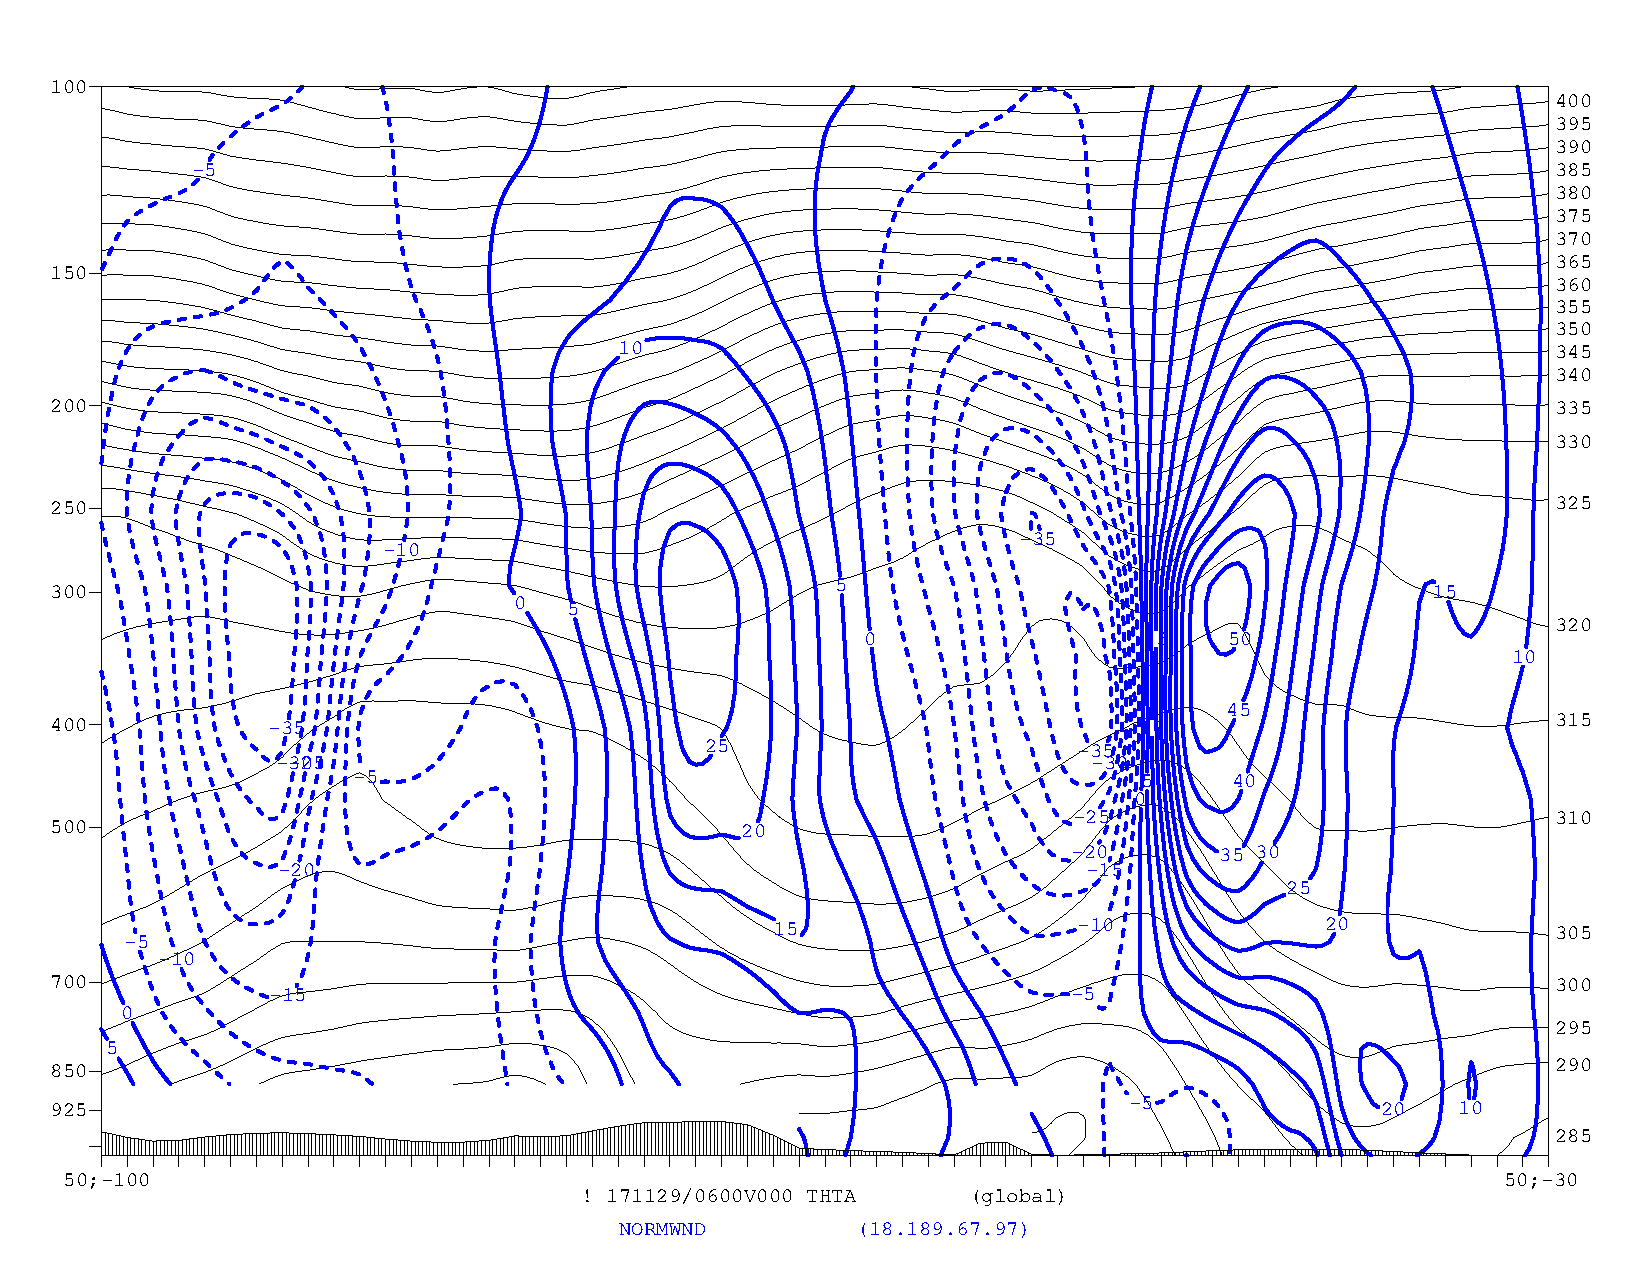
\includegraphics[width=\textwidth]{thta_normwnd_50N_zon_xsec} % ,trim={2.5cm 1cm 2.5cm 0},clip
	\caption{Zonal cross-section of potential temperature (contours in solid black) with meridional wind velocity contours superimposed in blue (solid for positive velocities, dashed for negative) at a latitude of \SI{50}{\degree N} from 100--\SI{30}{\degree W} on November 29, 2017.}
	\label{fig:thta_normwnd_50N_zon_xsec}
\end{figure}

\begin{figure}[h!]
	\centering
	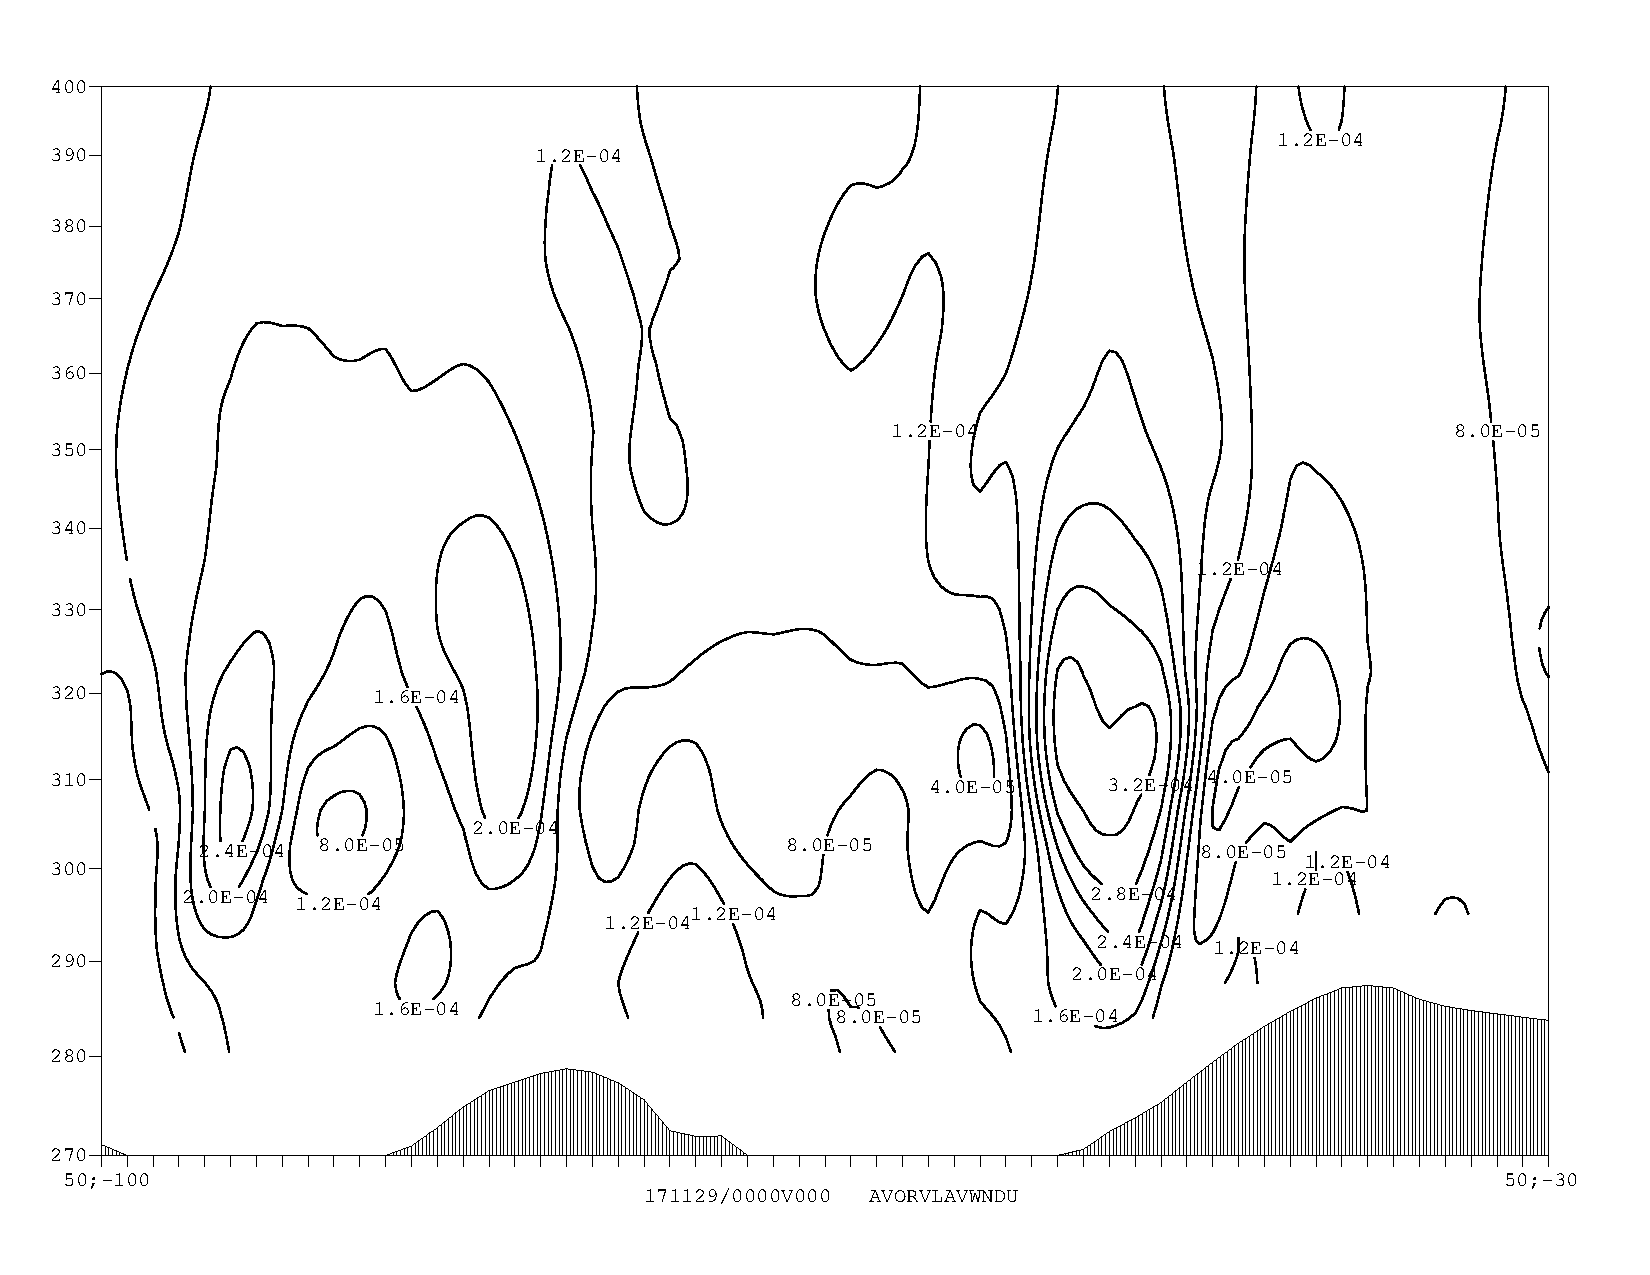
\includegraphics[width=\textwidth]{avor_theta_coord_50N_zon_xsec_0Z} % ,trim={2.5cm 1cm 2.5cm 0},clip
	\caption{Zonal cross-section of absolute vorticity (contours in solid black) at a latitude of \SI{50}{\degree N} from 100--\SI{30}{\degree W} on November 29, 2017.}
	\label{fig:avor_theta_coord_50N_zon_xsec_0Z}
\end{figure}

\begin{figure}[h!]
	\centering
	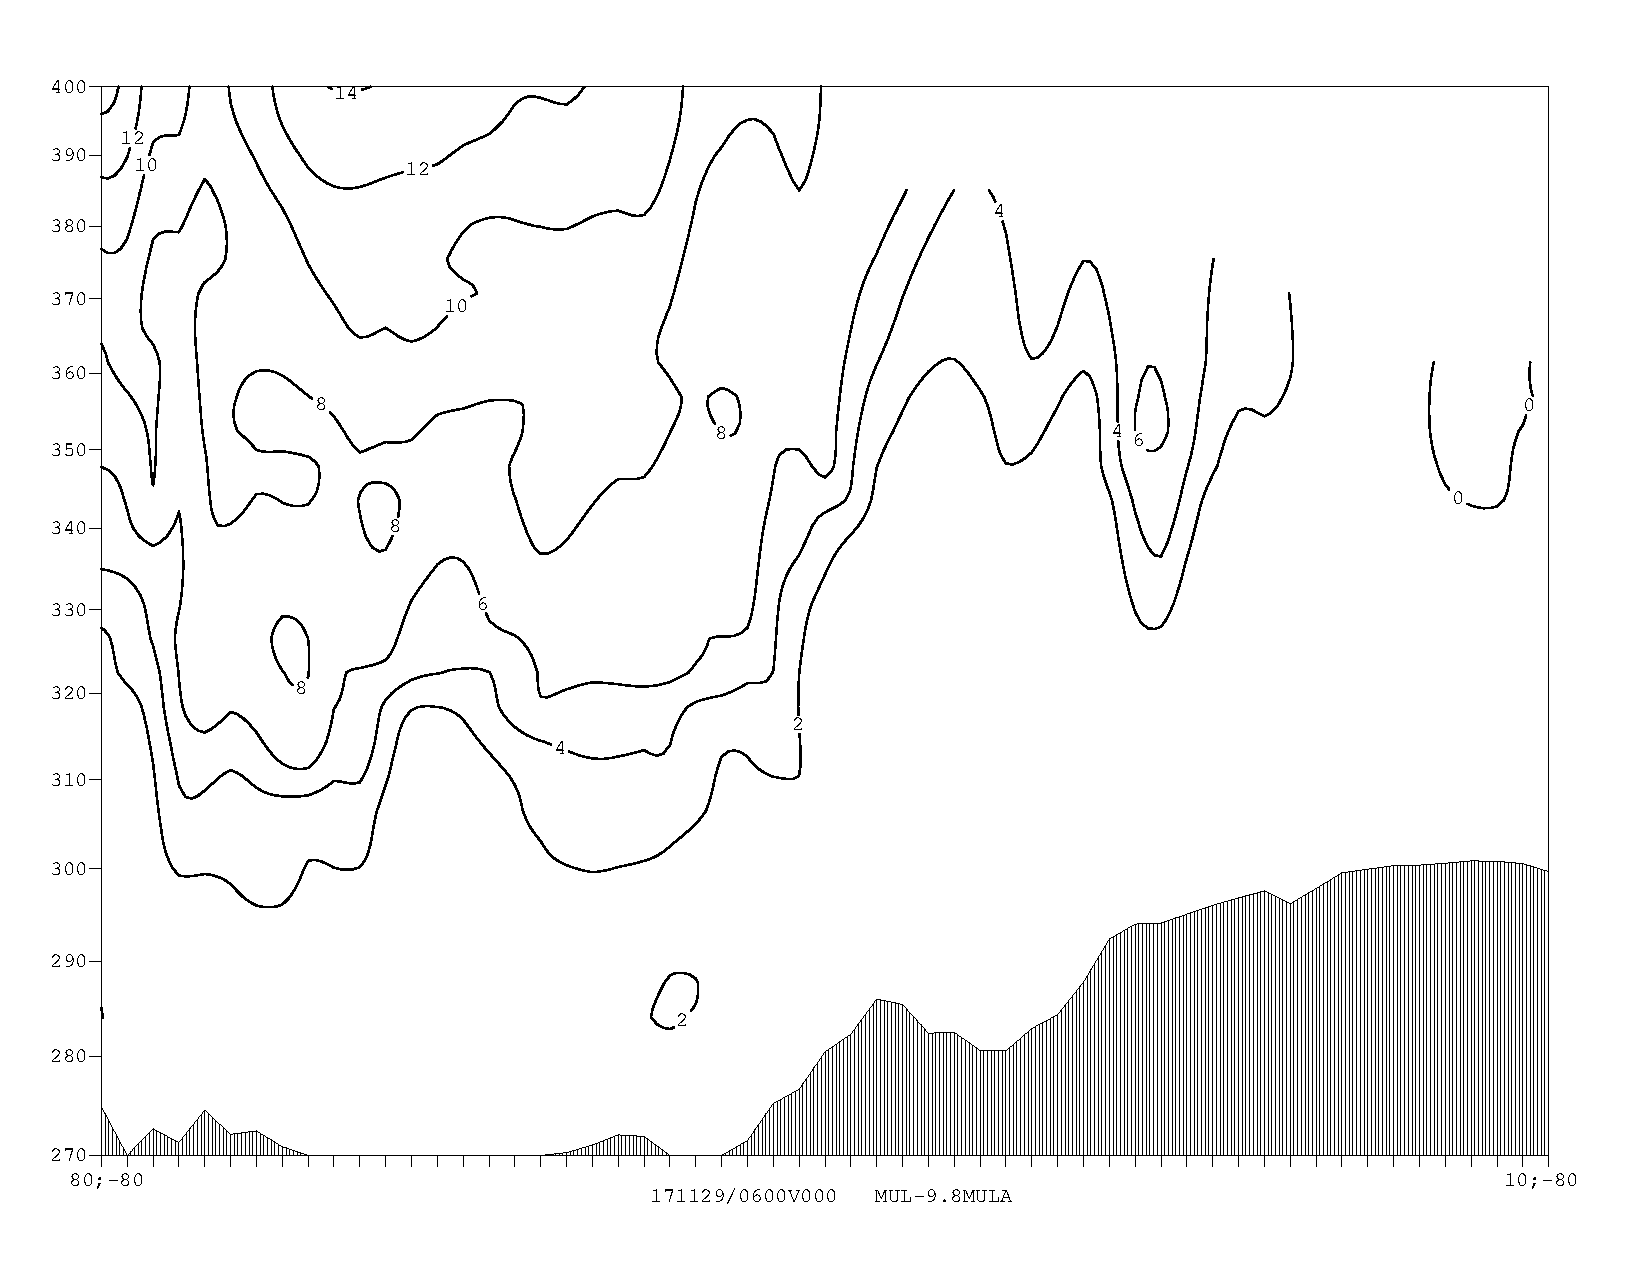
\includegraphics[width=\textwidth]{ipv_thta_coord_50N_zon_xsec_6Z_clearer_tropopause} % ,trim={2.5cm 1cm 2.5cm 0},clip
	\caption{Meridional cross-section of isentropic potential vorticity in potential temperature coordinates (contours in solid black) at a longitude of \SI{80}{\degree W} from 10--\SI{80}{\degree N} on November 29, 2017.}
	\label{fig:ipv_thta_coord_50N_zon_xsec_6Z}
\end{figure}

\begin{figure}[h!]
	\centering
	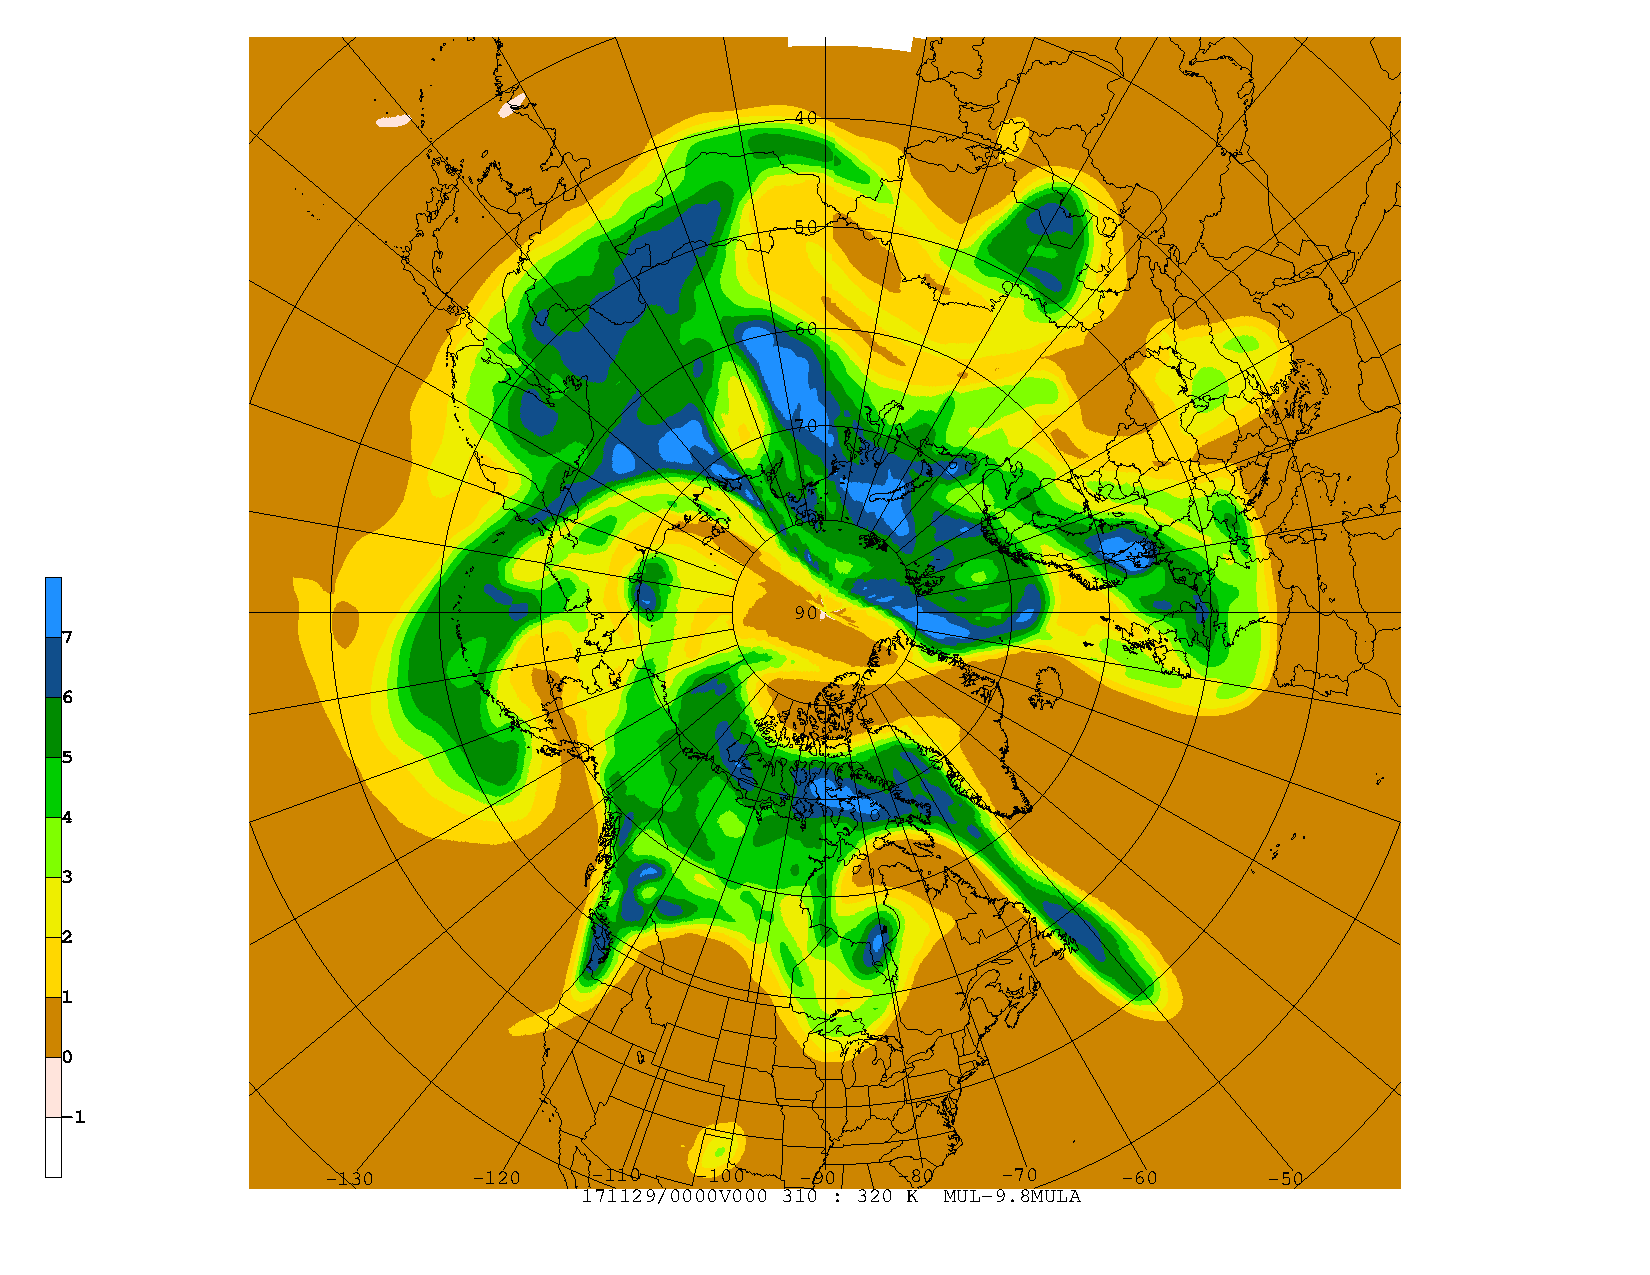
\includegraphics[width=\textwidth,trim={0cm 1cm 4cm 0.5cm},clip]{ipv_north_hemisphere_0Z}
	\caption{Contour plot of the isentropic potential vorticity field for potential temperatures of 310--320 K over the Northern Hemisphere on November 29, 2017.}
	\label{fig:ipv_north_hemisphere_0Z}
\end{figure}

We can compare our cross-sections with the climatologies provided by \url{http://synoptic.mit.edu/wp-content/uploads/2016/09/PV_climatology.pdf}. Of particular interest is the map of annual mean (1979--2001) potential temperature on the dynamical tropopause showing the extent of the tropopause at potential temperatures of 310--320 K. The climatological mean shows a very rounded tropopause structure circling the globe at around \SI{50}{\degree N}, bulging out over Canada in North America and Russia in Asia. The snapshot of the tropopause in figure \ref{fig:ipv_north_hemisphere_0Z} shows a very dynamic tropopause that much more structure and variability. It is bulging out not only over North America and Asia but also over the Pacific Ocean, almost reaching a latitude of \SI{40}{\degree N}. A noticable feature in the structure of the dynamical tropopause is the presence of long cold ``tongues'' where the tropopause sticks out into the lower latitudes. A few of them can be found in figure \ref{fig:ipv_north_hemisphere_0Z}, specifically through Baffin Bay down the west coast of Greenland and deep into the North Atlantic, and a smaller one extending south to Washington state. There are also a few isolated regions where the tropopause heights is depressed, noticeably over the Baltic Sea between Sweden and Poland and another one over Uzbekistan. In watching the evolution of the tropopause in the next section, these isolated spots seems to separate from the main tongues when it is extended far to the south and subsequently decay over a period of a couple of days.

Comparing the potential temperatures and wind velocities in figure \ref{fig:thta_normwnd_50N_zon_xsec} with climatological means, we see that the maximum wind speed occurs at a pressure of roughly 300 hPa which is slightly lower than the climatological mean. Of course, figure \ref{fig:thta_normwnd_50N_zon_xsec} gives the meridional wind speed while the climatological plot provides the zonal, however, if the wind is circulating around the tropopause height depression over the North Atlantic (see figure \ref{fig:ipv_north_hemisphere_0Z}) then we might expect roughly equal meridional and zonal wind speeds. We also see that the tropopause height occurs at roughly 330--340 K which agrees with the climatology for a latitude of \SI{50}{\degree N}.

From inspecting figure \ref{fig:avor_theta_coord_50N_zon_xsec_0Z} but especially figure \ref{fig:ipv_thta_coord_50N_zon_xsec_6Z}, we see that the tropopause coincides with the 315 K potential temperature surface, which agrees very well with the climatological zonal mean potential vorticity contour plot, which also suggests a tropopause height coinciding with $\theta = 315 \text{K}$ at a latitude of \SI{50}{\degree N}.

\section{Tropopause maps}
Figure \ref{fig:tropopause_map} shows the position of the tropopause over North America on December 3, 2017 (12Z) at various potential temperatures from 370--380 K to 290--300 K. We define the tropopause's position to be the 2 PVU surface. We can compare it with an automatically generated tropopause temperature maps, such as the one shown in figure \ref{fig:2017120312_US_tropo} which shows the position of the tropopause using the same definition at the same time as a function of potential temperature as colored contours along with 850 hPa saturation equivalent potential temperature contours in dashed black and surface pressure contours in solid black.

\begin{figure}[h!]
	\centering
	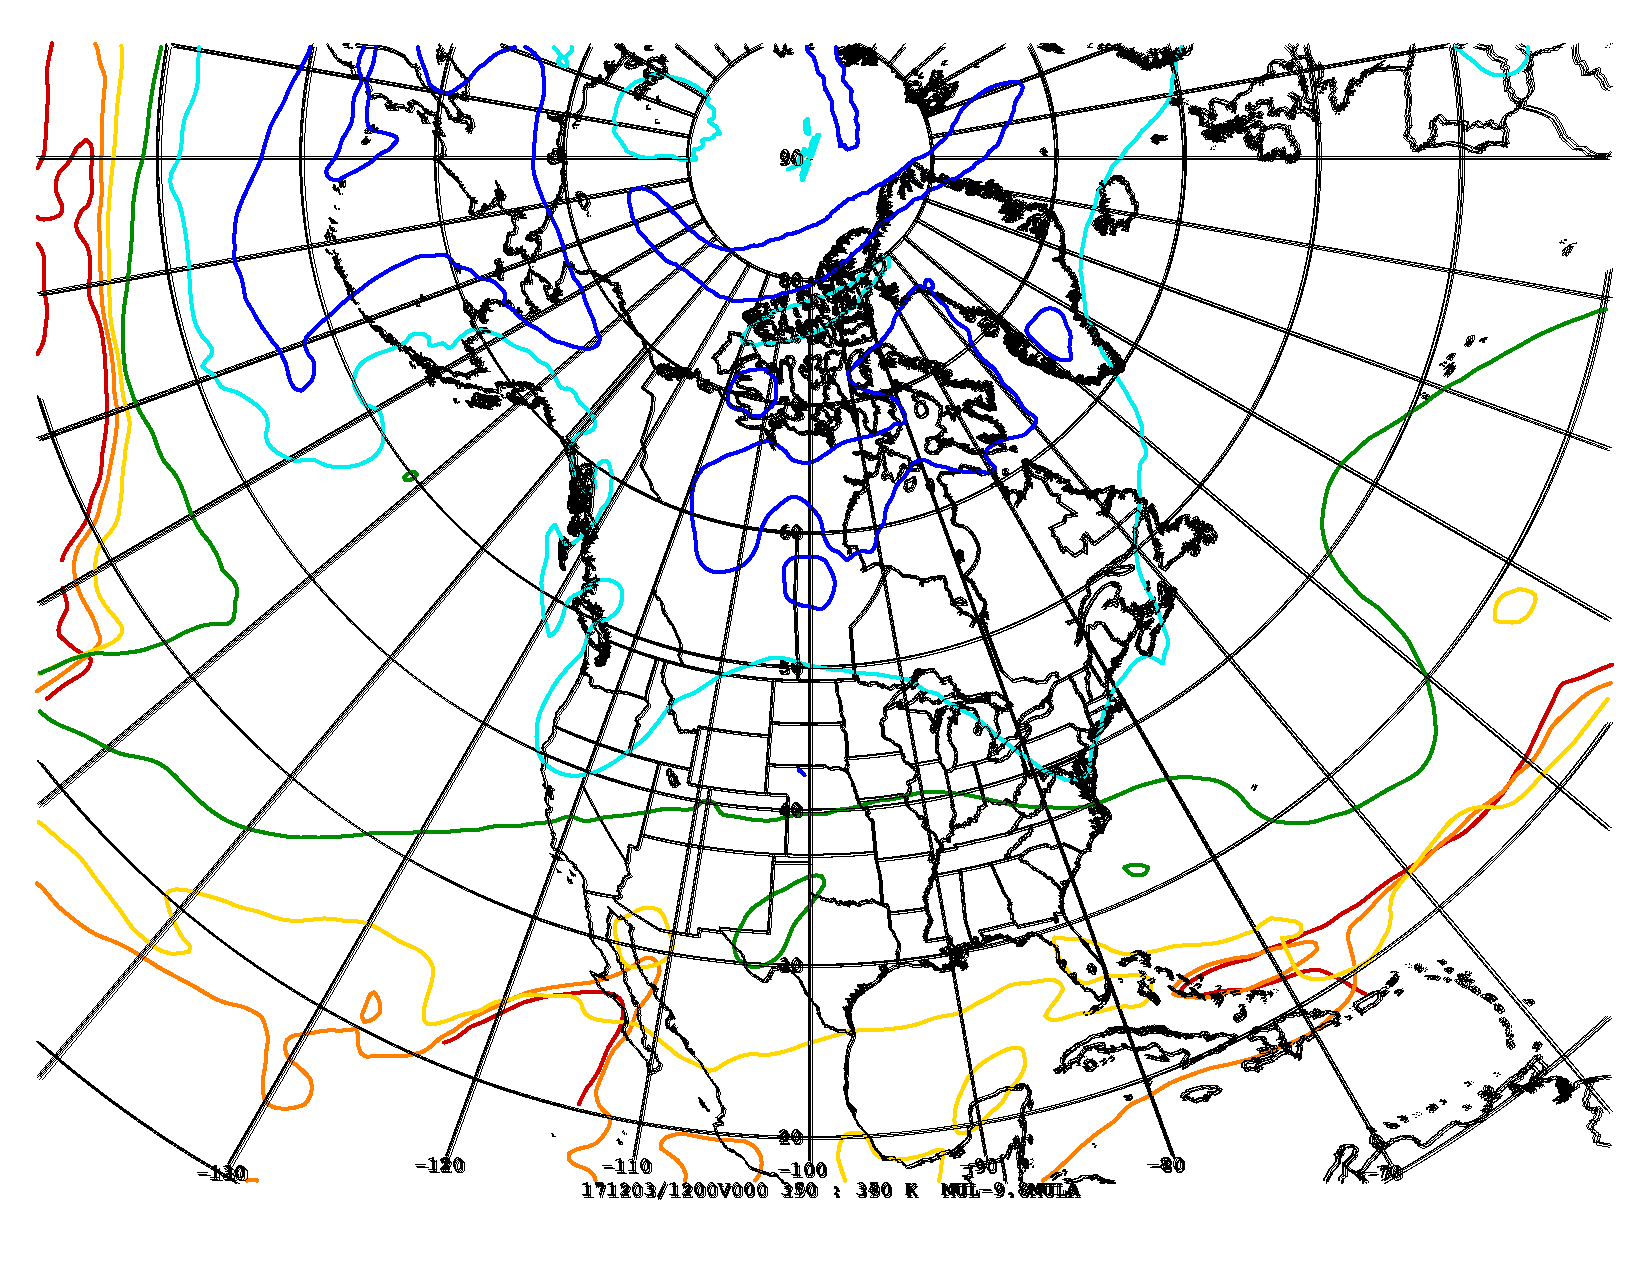
\includegraphics[width=\textwidth]{tropopause_map} % ,trim={2.5cm 1cm 2.5cm 0},clip
	\caption{The position of the tropopause (defined as the 2 PVU surface) over North America on December 3, 2017 (12Z) at various potential temperatures: 370--380 K in red, 360--370 K in orange, 350--360 K in yellow, 330--340 K in green, 310--320 K in cyan, 290-300 K in blue. Apologies for the lack of a color legend and for the non-overlapping borders as I merged each tropopause map manually.}
	\label{fig:tropopause_map}
\end{figure}

\begin{figure}[h!]
	\centering
	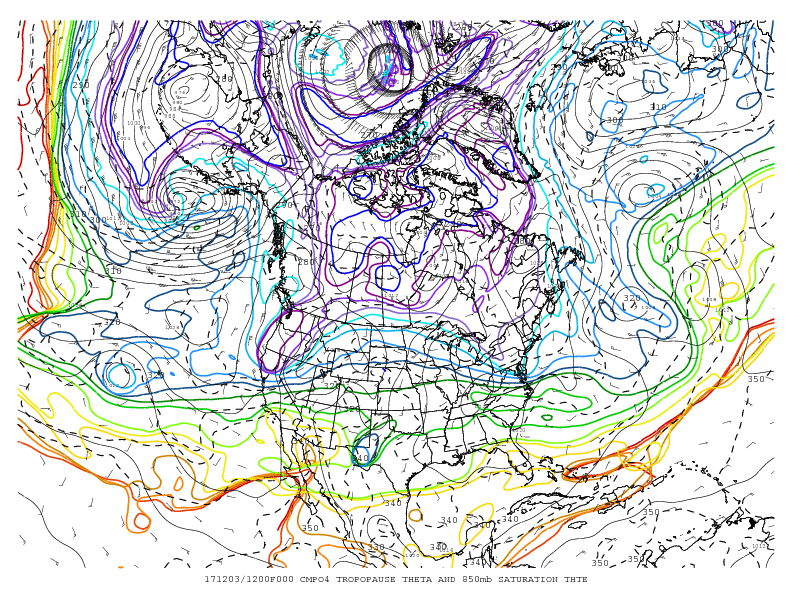
\includegraphics[width=\textwidth]{2017120312_US_tropo.png} % ,trim={2.5cm 1cm 2.5cm 0},clip
	\caption{The potential temperature on the dynamical tropopause (color contours), which is defined as the surface having potential vorticity $q$ of 2.0 PVU (1 PVU = $\SI{10e6}{\m\squared\K\per\kg\per\second}$).  The contour interval of potential temperature is 5 K, with the most extreme purple being 280 K and the most extreme red 375 K. Also shown are the 850 hPa saturation equivalent potential temperature (dashed black contours, with contour interval of 5 K) and the surface pressure (solid black contours, labelled in hPa).}
	\label{fig:2017120312_US_tropo}
\end{figure}

The comparison can be a little tough due to the lower resolution and additional information provided in the full tropopause map in figure \ref{fig:2017120312_US_tropo}, but we can utilize the fact that they use the same colormap for the potential temperature surface contours. We see that the contours in our reproduction (figure \ref{fig:tropopause_map}) closely resemble the full tropopause map in figure \ref{fig:2017120312_US_tropo}. The full figure shows a clearer picture of the tropopause as it plots the surface pressures as well, so we can see a couple of low pressure systems, such as the one southwest of Alaska, coinciding with lower tropopause heights.

\section{A case study}
For this case study we will be referring to the tropopause evolution maps for the 310--320 K potential temperature surface from \url{http://synoptic.mit.edu/wp-content/uploads/2016/09/trop_maps_171203-04.pdf}. It provides the height of the 2 PVU tropopause at various potential temperature surfaces on December 3, 2017 (12Z) and December 4, 2017 (12Z). It also provides snapshots of the 2 PVU tropopause from December 3, 2017 (12Z) to December 6, 2017 (12Z) in 12-hour intervals as well as the evolution of the tropopause on the 850 hPa saturation $\theta_e$ surface where $\theta_e$ is the equivalent potential temperature. By simply referring to the figures, we will avoid having to reprint 25 figures.

Comparing the 2 PVU tropopause height from December 3--4 we see that the tropopause height has shifted southward a little towards the continental United States except at low potential temperature surfaces, and it has noticeably moved eastward at low potential temperature surfaces over Northern Canada. For the 290--320 K surfaces, the ``tongues'' seem more pronounced and appear to stretch southward over the time period as well. Looking at the evolution of the 310--320 K potential surface temperature surface in cyan, we can see the tropopause height structure moving eastward, almost traversing the continental United States between December 3 and 6 (12Z) as indicated by the moving tongue from Washington to Quebec. The tongues arise from baroclinic instabilities and also extend southward as the system evolves in time, reaching as far south as Southern California and the \SI{30}{\degree N} latitude line over the Pacific. This would bring cold air down to these regions.

Looking at the surface temperature and tropopause temperature undulations at 850 hPa over the same period, we see that the two undulate very closely in phase with only a few anomalies such as over the Pacific Ocean on December 4, 2017 (12Z).

According to thermal wind balance, a low tropopause is accompanied by a cyclone as we know that it brings warm southerly winds northward in the Northern Hemisphere. Thus a high tropopause would induce an anti-cyclone.

% Would you expect a cold surface to induce cyclonic or anticyclonic circulation? Draw a sketch. What about a warm surface?

\end{document}